%%% Research Diary - Entry
%%% Template by Mikhail Klassen, April 2013
%%% 
\documentclass[11pt,letterpaper]{article}

\newcommand{\workingDate}{\textsc{2013 $|$ January $|$ 01}}
\newcommand{\userName}{Lars-Hendrik Frahm}
\newcommand{\institution}{Universit\"at Hamburg}
\usepackage{researchdiary_png}
\usepackage{braket}
\usepackage{tikz}
\usepackage{graphicx}               % Necessary to use \scalebox
\usepackage{amsmath,amssymb}
\usetikzlibrary{calc,intersections}
\usetikzlibrary{matrix,calc}

\def\r{0.7cm}
\def\mpstensor(#1,#2,#3,#4,#5,#6,#7){
  \node[draw, shape=circle, minimum size=#1, inner sep=0pt] (tns_dn) at (#2,#3) {#4};
  \draw [thick] (tns_dn.west) -- (#2-#1,#3) node[left] {\tiny{#5}};
  \draw [thick] (tns_dn.east) -- (#2+1*#1,#3) node[right] {\tiny{#6}};
  \draw [thick] (tns_dn.north) -- (#2,#3+1*#1) node[above] {\tiny{#7}};
}

\def\mpstensorT(#1,#2,#3,#4,#5,#6,#7){
  \node[draw, shape=circle, minimum size=#1, inner sep=0pt] (tns_dn) at (#2,#3) {#4};
  \draw [thick] (tns_dn.west) -- (#2-1*#1,#3) node[left] {\tiny{#5}};
  \draw [thick] (tns_dn.east) -- (#2+1*#1,#3) node[right] {\tiny{#6}};
  \draw [thick] (tns_dn.south) -- (#2,#3-1*#1) node[below] {\tiny{#7}};
}

\def\tensorOR(#1,#2,#3,#4,#5,#6){
  \node[draw, shape=rectangle, minimum height=2.5*#1, minimum width=#1, inner sep=0pt, rounded corners, name path=yborder] (tns) at (#2,#3) {#4};
  \path [name path=lower ] (#2+0.5*#1,#3-0.8*#1) -- (#2+0.5*#1+0.5*#1,#3-0.8*#1);
  \path [name path=upper ] (#2+0.5*#1,#3+0.8*#1) -- (#2+0.5*#1+0.5*#1,#3+0.8*#1);
  \draw [name intersections={of=yborder and lower}, thick]
                             (intersection-1) -- ++(0.5*#1,0)node[right] {\tiny{#6}};
  \draw [name intersections={of=yborder and upper}, thick]
                             (intersection-1) -- ++(0.5*#1,0) node[right] {\tiny{#5}};                             
}
\def\tensorOL(#1,#2,#3,#4,#5,#6){
  \node[draw, shape=rectangle, minimum height=2.5*#1, minimum width=#1, inner sep=0pt, rounded corners, name path=yborder] (tns) at (#2,#3) {#4};
  \path [name path=lower ] (#2-0.5*#1,#3-0.8*#1) -- (#2-0.5*#1-0.5*#1,#3-0.8*#1);
  \path [name path=upper ] (#2-0.5*#1,#3+0.8*#1) -- (#2-0.5*#1-0.5*#1,#3+0.8*#1);
  \draw [name intersections={of=yborder and lower}, thick]
                             (intersection-1) -- ++(-0.5*#1,0)node[left] {\tiny{#6}};
  \draw [name intersections={of=yborder and upper}, thick]
                             (intersection-1) -- ++(-0.5*#1,0) node[left] {\tiny{#5}};                             
}
\begin{document}

\title{Tensor Note Book As in HamMPS}

{\Huge Tensor Notes}\\[5mm]

\section*{The Matrix Product State Tensor}

Using $SU(2)$ symmetry, $U(1)$ symmetry and point group symmetry all tensors in the matrix product state can be written as
\begin{align}
A[i]^{(ss^zNI)}_{(j_Lj^z_LN_LI_L\alpha_L);(j_Rj^z_RN_RI_R\alpha_R)} &= \braket{j_Lj^z_Lss^z|j_Rj^z_R}\delta_{N_L+N,N_R}\delta_{I_L\otimes I, I_R}\underbrace{T[i]^{(sNI)}_{(j_LN_LI_L\alpha_L);(j_RN_RI_R\alpha_R)}}_{\text{reduced Tensor}}\\
\begin{tikzpicture}[baseline=-0.5ex]
\mpstensor(0.8cm,0,0,$A[i]$,$j_Lj^z_LN_LI_L\alpha_L$,$j_Rj^z_RN_RI_R\alpha_R$,$ss^zNI$)
\end{tikzpicture} &= \braket{j_Lj^z_Lss^z|j_Rj^z_R}\delta_{N_L+N,N_R}\delta_{I_L\otimes I, I_R} \begin{tikzpicture}[baseline=-0.5ex]
\mpstensor(0.8cm,0,0,$T[i]$,$j_LN_LI_L\alpha_L$,$j_RN_RI_R\alpha_R$,$sNI$)
\end{tikzpicture}
\end{align}

Only the reduced Tensors $T[i]$ are used in the program. The actual tensors $A[i]$ are never stored in the memory
\section*{Overlap}
\subsection*{Left to Right}
\subsubsection*{Create New}
\begin{align}
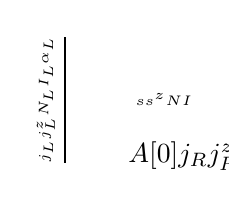
\begin{tikzpicture}[baseline=0.7cm]
\draw[thick] (-0.8,0.0) -- node[above, rotate=90] {\tiny{$j_Lj^z_LN_LI_L\alpha_L$}} (-0.8,1.6);
\node at (0.45, 0.8) {\tiny{$ss^zNI$}};
\mpstensorT(0.8cm,0,1.6cm,$A[0]$,,$j_Rj^z_RN_RI_R\alpha_R$,)
\mpstensor(0.8cm,0,0.0,$B[0]$,,$\tilde{j}_R\tilde{j}^z_R\tilde{N}_R\tilde{I}_R\tilde{\alpha}_R$,)
\end{tikzpicture} &= \sum_{\substack{ss^zNI \\ j_Lj^z_LN_LI_L\alpha_L}} \left( A[0]^{(ss^zNI)}_{(j_Lj^z_LN_LI_L\alpha_L);(j_Rj^z_RN_RI_R\alpha_R)} \right)^{\dagger}B[0]^{(ss^zNI)}_{(j_Lj^z_LN_LI_L\alpha_L);(\tilde{j}_R\tilde{j}^z_R\tilde{N}_R\tilde{I}_R\tilde{\alpha}_R)} \\
& = \delta_{j_R\tilde{j}_R}\delta_{j^z_R\tilde{j}^z_R}\delta_{N_R\tilde{N}_R}\delta_{I_R\tilde{I}_R}\nonumber\\&\ \ \ \sum_{\substack{sNI \\ j_LN_LI_L\alpha_L}} \left( T[0]^{(sNI)}_{(j_LN_LI_L\alpha_L);(j_RN_RI_R\alpha_R)} \right)^{\dagger}S[0]^{(sNI)}_{(j_LN_LI_L\alpha_L);(j_RN_RI_R\tilde{\alpha}_R)} \\
&= \delta_{j_R\tilde{j}_R}\delta_{j^z_R\tilde{j}^z_R}\delta_{N_R\tilde{N}_R}\delta_{I_R\tilde{I}_R}\underbrace{\sum_{\substack{sNI \\ j_LN_LI_L\alpha_L}}
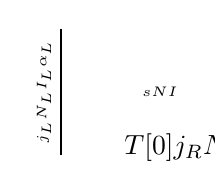
\begin{tikzpicture}[baseline=0.7cm]
\draw[thick] (-0.8,0.0) -- node[above, rotate=90] {\tiny{$j_LN_LI_L\alpha_L$}} (-0.8,1.6);
\node at (0.45, 0.8) {\tiny{$sNI$}};
\mpstensorT(0.8cm,0,1.6cm,$T[0]$,,$j_RN_RI_R\alpha_R$,)
\mpstensor(0.8cm,0,0.0,$S[0]$,,$j_RN_RI_R\tilde{\alpha}_R$,)
\end{tikzpicture}}_{O[0]}
\end{align}
\begin{align}
&= \delta_{j_R\tilde{j}_R}\delta_{j^z_R\tilde{j}^z_R}\delta_{N_R\tilde{N}_R}\delta_{I_R\tilde{I}_R} \ 
\begin{tikzpicture}[baseline=0.0cm]
\tensorOR(0.8cm, 0.0,0.0,$O[0]$,$j_RN_RI_R\alpha_R$,$j_RN_RI_R\tilde{\alpha}_R$)
\end{tikzpicture}
\end{align}
\subsubsection*{Update}

\begin{align}
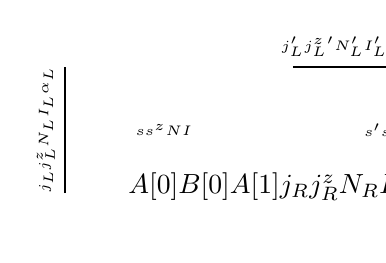
\begin{tikzpicture}[baseline=0.7cm]
\draw[thick] (-0.8,0.0) -- node[above, rotate=90] {\tiny{$j_Lj^z_LN_LI_L\alpha_L$}} (-0.8,1.6);
\node at (0.45, 0.8) {\tiny{$ss^zNI$}};
\mpstensorT(0.8,0,1.6,$A[0]$,,,)
\mpstensor(0.8,0,0.0,$B[0]$,,,)
\node at (2.25, 0.8) {\tiny{$s'{s'}^{z}N'I'$}};
\draw[thick] (0.8, 1.6) -- node[above]{\tiny{$j'_L{j^z_L}'{N'_L}{I'_L}{\alpha'_L}$}} (2.2, 1.6);
\mpstensorT(0.8,3.0,1.6,$A[1]$,,$j_Rj^z_RN_RI_R\alpha_R$,)
\mpstensor(0.8,3.0,0.0,$B[1]$,,$\tilde{j}_R\tilde{j}^z_R\tilde{N}_R\tilde{I}_R\tilde{\alpha}_R$,)
\draw[thick] (0.8, 0.0) -- node[below]{\tiny{${\tilde{j}_L}'\tilde{j^z_L}'{\tilde{N}_L}'{\tilde{I}_L}'{\tilde{\alpha}_L}'$}} (2.2, 0.0);
\end{tikzpicture} \hspace{-2em}= \delta_{j_R\tilde{j}_R}\delta_{j^z_R\tilde{j}^z_R}\delta_{N_R\tilde{N}_R}\delta_{I_R\tilde{I}_R}\sum_{\substack{sNI \\ j_LN_LI_L\alpha_L\tilde{\alpha}_L}}
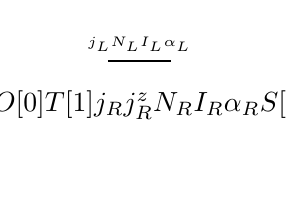
\begin{tikzpicture}[baseline=0.0cm]
\tensorOR(0.8cm, 0.0,0.0,$O[0]$,,)
\draw[thick] (0.8,0.640) -- node[above] {\tiny{$j_LN_LI_L\alpha_L$}} (1.6,0.640);
\mpstensorT(0.8,2.4,0.640,$T[1]$,,$j_Rj^z_RN_RI_R\alpha_R$,)
\node at (2.9, 0.0) {\tiny{$s{s}^{z}NI$}};
\mpstensor(0.8,2.4,-0.640,$S[1]$,,$j_Rj^z_RN_RI_R\tilde{\alpha}_R$,)
\draw[thick] (0.8,-0.640) -- node[below] {\tiny{$j_LN_LI_L\tilde{\alpha}_L$}} (1.6,-0.640);
\end{tikzpicture}
\end{align}
\begin{align}
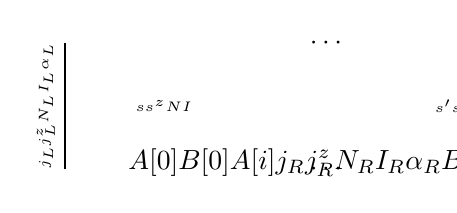
\begin{tikzpicture}[baseline=0.7cm]
\draw[thick] (-0.8,0.0) -- node[above, rotate=90] {\tiny{$j_Lj^z_LN_LI_L\alpha_L$}} (-0.8,1.6);
\node at (0.45, 0.8) {\tiny{$ss^zNI$}};
\mpstensorT(0.8,0,1.6,$A[0]$,,,)
\mpstensor(0.8,0,0.0,$B[0]$,,,)
\node at (1.25, 1.6) {$\cdots$};
\node at (1.25, 0.0) {$\cdots$};
\node at (3.15, 0.8) {\tiny{$s'{s'}^{z}N'I'$}};
\mpstensorT(0.8,2.5,1.6,$A[i]$,,$j_Rj^z_RN_RI_R\alpha_R$,)
\mpstensor(0.8,2.5,0.0,$B[i]$,,$\tilde{j}_R\tilde{j}^z_R\tilde{N}_R\tilde{I}_
R\tilde{\alpha}_R$,)
\end{tikzpicture} \hspace{-2em}&= \delta_{j_R\tilde{j}_R}\delta_{j^z_R\tilde{j}^z_R}\delta_{N_R\tilde{N}_R}\delta_{I_R\tilde{I}_R}\sum_{\substack{sNI \\ j_LN_LI_L\alpha_L\tilde{\alpha}_L}}
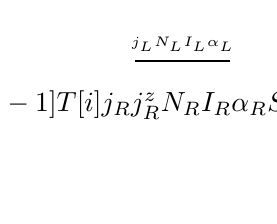
\begin{tikzpicture}[baseline=0.0cm]
\tensorOR(0.8cm, 0.0,0.0,$O[i-1]$,,)
\draw[thick] (1.0,0.640) -- node[above] {\tiny{$j_LN_LI_L\alpha_L$}} (2.2,0.640);
\mpstensorT(0.8,2.8,0.640,$T[i]$,,$j_Rj^z_RN_RI_R\alpha_R$,)
\node at (3.3, 0.0) {\tiny{$sNI$}};
\mpstensor(0.8,2.8,-0.640,$S[i]$,,$j_Rj^z_RN_RI_R\tilde{\alpha}_R$,)
\draw[thick] (1.0,-0.640) -- node[below] {\tiny{$j_LN_LI_L\tilde{\alpha}_L$}} (2.2,-0.640);
\end{tikzpicture} \\
&= \delta_{j_R\tilde{j}_R}\delta_{j^z_R\tilde{j}^z_R}\delta_{N_R\tilde{N}_R}\delta_{I_R\tilde{I}_R}\sum_{\substack{sNI \\ j_LN_LI_L\alpha_L\tilde{\alpha}_L}}\left( T[i]^{(sNI)}_{(j_LN_LI_L\alpha_L);(j_RN_RI_R\alpha_R)} \right)^{\dagger} \nonumber\\
&\hspace{4em} O[i-1]_{(j_LN_LI_L\alpha_L);(j_LN_LI_L\tilde{\alpha}_L)} S[i]^{(sNI)}_{(j_LN_LI_L\tilde{\alpha}_L);(j_RN_RI_R\tilde{\alpha}_R)}
\end{align}
\subsection*{Right to Left}
\subsubsection*{Create New}
\begin{align}
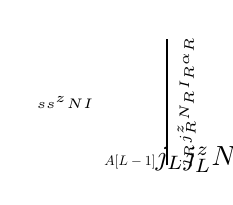
\begin{tikzpicture}[baseline=0.7cm]
\draw[thick] (0.8,0.0) -- node[below, rotate=90] {\tiny{$j_Rj^z_RN_RI_R\alpha_R$}} (0.8,1.6);
\node at (-0.5, 0.8) {\tiny{$ss^zNI$}};
\mpstensorT(0.8cm,0,1.6cm,\scalebox{.5}{$A[L-1]$},$j_Lj^z_LN_LI_L\alpha_L$,,)
\mpstensor(0.8cm,0,0.0,\scalebox{.5}{$B[L-1]$},$\tilde{j}_L\tilde{j}^z_L\tilde{N}_L\tilde{I}_L\tilde{\alpha}_L$,,)
\end{tikzpicture} &= \sum_{\substack{ss^zNI \\ j_Rj^z_RN_RI_R\alpha_R}} A[L-1]^{(ss^zNI)}_{(j_Lj^z_LN_LI_L\alpha_L);(j_Rj^z_RN_RI_R\alpha_R)} \left( B[L-1]^{(ss^zNI)}_{(\tilde{j}_L\tilde{j}^z_L\tilde{N}_L\tilde{I}_L\tilde{\alpha}_L);(j_Rj^z_RN_RI_R\alpha_R)} \right)^{\dagger} \\
& = \scriptstyle{ \delta_{j_L\tilde{j}_L}\delta_{j^z_L\tilde{j}^z_L}\delta_{N_L\tilde{N}_L}\delta_{I_L\tilde{I}_L}\nonumber}\\&\ \ \ \scriptstyle {\sum_{\substack{sNI \\ j_RN_RI_R\alpha_R}} \frac{2j_R+1}{2j_L+1} T[L-1]^{(sNI)}_{(j_RN_RI_R\alpha_R);(j_RN_RI_R\alpha_R)} \left ( S[L-1]^{(sNI)}_{(j_LN_LI_L\tilde{\alpha}_L);(j_RN_RI_R\tilde{\alpha}_R)} \right)^{\dagger} } \\
&= \delta_{j_L\tilde{j}_L}\delta_{j^z_L\tilde{j}^z_L}\delta_{N_L\tilde{N}_L}\delta_{I_L\tilde{I}_L}\sum_{\substack{sNI \\ j_LN_LI_L\alpha_L}}\frac{2j_R+1}{2j_L+1}
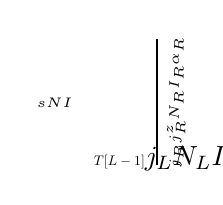
\begin{tikzpicture}[baseline=0.7cm]
\draw[thick] (0.8,0.0) -- node[below, rotate=90] {\tiny{$j_Rj^z_RN_RI_R\alpha_R$}} (0.8,1.6);
\node at (-0.5, 0.8) {\tiny{$sNI$}};
\mpstensorT(0.8cm,0,1.6cm,\scalebox{.5}{$T[L-1]$},$j_LN_LI_L\alpha_L$,,)
\mpstensor(0.8cm,0,0.0,\scalebox{.5}{$S[L-1]$},$j_LN_LI_L\tilde{\alpha}_L$,,)
\end{tikzpicture}
\end{align}
\begin{align}
&= \delta_{j_L\tilde{j}_L}\delta_{j^z_L\tilde{j}^z_L}\delta_{N_L\tilde{N}_L}\delta_{I_L\tilde{I}_L} \ 
\begin{tikzpicture}[baseline=0.0cm]
\tensorOL(0.8cm, 0.0,0.0,$\scalebox{.5}{$O[L-1]$}$,$j_RN_RI_R\alpha_R$,$j_RN_RI_R\tilde{\alpha}_R$)
\end{tikzpicture}
\end{align}
\subsubsection*{Update}

\begin{align}
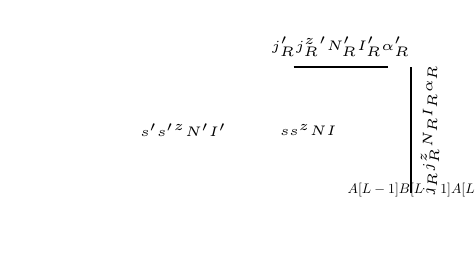
\begin{tikzpicture}[baseline=0.7cm]
\draw[thick] (0.8,0.0) -- node[below, rotate=90] {\tiny{$j_Rj^z_RN_RI_R\alpha_R$}} (0.8,1.6);
\node at (-0.5, 0.8) {\tiny{$ss^zNI$}};
\mpstensorT(0.8,0,1.6,\scalebox{.5}{$A[L-1]$},,,)
\mpstensor(0.8,0,0.0,\scalebox{.5}{$B[L-1]$},,,)
\draw[thick] (-2.0, 1.6) -- node[above]{\tiny{$j'_R{j^z_R}'{N'_R}{I'_R}{\alpha'_R}$}} (-0.8, 1.6);
\node at (-3.4, 0.8) {\tiny{$s'{s'}^{z}N'I'$}};
\mpstensorT(0.8,-2.8,1.6,\scalebox{.5}{$A[L-2]$},$j_Lj^z_LN_LI_L\alpha_L$,,)
\mpstensor(0.8,-2.8,0.0,\scalebox{.5}{$B[L-2]$},$\tilde{j}_R\tilde{j}^z_R\tilde{N}_R\tilde{I}_R\tilde{\alpha}_R$,,)
\draw[thick] (-2.0, 0.0) -- node[below]{\tiny{${\tilde{j}_R}'\tilde{j^z_R}'{\tilde{N}_R}'{\tilde{I}_R}'{\tilde{\alpha}_R}'$}} (-0.8, 0.0);
\end{tikzpicture}
= &\delta_{j_L\tilde{j}_L}\delta_{j^z_L\tilde{j}^z_L}\delta_{N_L\tilde{N}_L}\delta_{I_L\tilde{I}_L}\sum_{\substack{sNI \\ j_RN_RI_R\alpha_R\tilde{\alpha}_R}} \frac{2j_R+1}{2j_L+1} \nonumber\\
& \hspace{4em}
\begin{tikzpicture}[baseline=0.0cm]
\tensorOL(0.8cm, 0.0,0.0,$\scalebox{.5}{$O[L-1]$}$,,)
\draw[thick] (-0.8,0.640) -- node[above] {\tiny{$j_RN_RI_R\alpha_R$}} (-1.6,0.640);
\mpstensorT(0.8,-2.4,0.640,$\scalebox{.5}{$T[L-2]$}$,$j_Lj^z_LN_LI_L\alpha_L$,,)
\node at (-2.7, 0.0) {\tiny{$sNI$}};
\mpstensor(0.8,-2.4,-0.640,$\scalebox{.5}{$S[L-2]$}$,$j_Lj^z_LN_LI_L\tilde{\alpha}_L$,,)
\draw[thick] (-0.8,-0.640) -- node[below] {\tiny{$j_RN_RI_R\tilde{\alpha}_R$}} (-1.6,-0.640);
\end{tikzpicture} \\
= &\delta_{j_L\tilde{j}_L}\delta_{j^z_L\tilde{j}^z_L}\delta_{N_L\tilde{N}_L}\delta_{I_L\tilde{I}_L}\sum_{\substack{sNI \\ j_RN_RI_R\alpha_R\tilde{\alpha}_R}} \frac{2j_R+1}{2j_L+1} \nonumber\\
& T[L-2]^{(sNI)}_{(j_LN_LI_L\alpha_L);(j_RN_RI_R\alpha_R)} O[L-1]_{(j_RN_RI_R\alpha_R);(j_RN_RI_R\tilde{\alpha}_R)} \nonumber\\
&\hspace{4em}\left ( S[L-1]^{(sNI)}_{(j_LN_LI_L\tilde{\alpha}_L);(j_RN_RI_R\tilde{\alpha}_R)} \right)^{\dagger}
\end{align}

\section*{Annihilation Operator}
\subsection*{Left to Right}
\end{document}
